\documentclass[12pt]{article}
\usepackage[margin=1in]{geometry}
\usepackage{amsmath}
\usepackage{amssymb}
\usepackage{setspace}
\usepackage{graphicx}
\usepackage{cite}

\usepackage{sectsty}

\sectionfont{\fontsize{12}{15}\selectfont}
\subsectionfont{\fontsize{12}{15}\selectfont}
\vspace{-30em}

\vspace{-2em}
\begin{document}
\vspace{-3em}
\small Natural Computing Assessment 


\small Exam Nos. B156771, B189288
\section{Neural Network Training with PSO}
\subsection{Choosing the Fitness Function}
This task is interpreted to mean that we are to design a fitness function to evaluate the fitness of the network as a whole after it has been trained.
Let the training error be $e_{train}$, and the testing error $e_{test}$. 
Taking the average of the two would be a sensible, if not standard course of action. 
However, a fitness function would need to incorporate a measure of how overfit the model is to the training data in order to be effective. 
In this sense, adding the difference between the two values is simple and effective. 
Ultimately, the fitness function takes the following form:
\begin{equation}
    f(e_{train}, e_{test}) = 1 - \left(\frac{e_{train} + e_{test}}{2} + \left(e_{test} - e_{train}\right)\right),
\end{equation}
where the error is calculated using the Mean Squared Error function. We subtract the average and distance from 1 to ensure that a greater fitness value implies a better model.

\subsection{Defining the Search Space}
The search space of a PSO is given by $[a,b]^D$, where $a,b\in \mathbb{R}$, and $D\in\mathbb{N}$ is the dimension of the space. 
We define the shape of a neural network by a sequence $(a_n)_{n=1}^{l}$ where $l\in\mathbb{N}$ defines the number of layers, and each $a_n \in \mathbb{N}$ gives the number of neurons in layer $n$. 
The dimension of the weight vector for $a$ would be the number of edges and nodes minus the input and output nodes. More simply:
\begin{equation}
    D = \left(\sum_{i=1}^{l-1} a_{n+1}\left(a_n + 1\right)\right) - a_l,
\end{equation}
where the final decrement addresses non-existent bias terms in the output layer that were counted in the summation. For this task, we set the shape to be $\left(6, 8, 1\right)$, meaning that the dimension of the search space $D=43$. 
To ensure that we are notified of a divergent swarm, we set $-a=b=20$, meaning that the search space for the PSO will be $\left[-20,20\right]^{43}$. 

\subsection{Training the Model}
For this task we trained two neural networks: one using Particle Swarm as its optimiser, and another using Stochastic Gradient Descent.
The model using SGD provides a fairly standard baseline on which to test the PSO model. 
% In the code provided, the PSO neural net does not use any third party machine learning libraries, as due to the nature of PSO, these neural nets only needed to consider forward propagation, not backwards.
% For the SGD optimised net, Pytorch was used due to the myriad of material online explaining how to code it. 
Each network was trained with 2-fold cross validation using the cross-validate program provided (refer to the README in the task-1 directory on how to use it). 
We chose 2 folds to more closely follow the instructions outlined in the assignment. A higher number of folds is feasible but tends to yield lower fitness values.
The parameters for the PSO were as follows: $n=20$, $\omega=0.7$, $\alpha_1 = 1.5 = \alpha_2 = 1.3$. 
The parameters for the SGD were as follows: learning rate $=0.03$.
The figure below shows the training and testing loss of both over time:

\begin{figure}[h]                   
      \begin{center}                  
          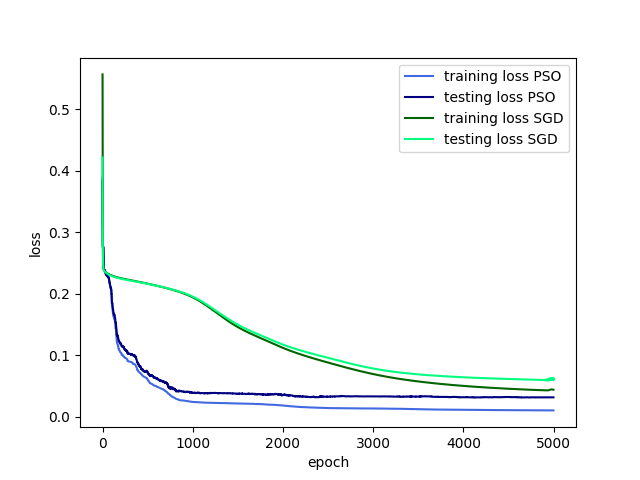
\includegraphics[scale=0.45]{figures/nonlinear.png}    
      \end{center}                                                                             
\end{figure}
The table in appendix A.1 shows the final average training and testing losses, as well as the average fitness using equation (1).

By these results it would appear that the model trained using PSO as its optimiser performed slightly better than the model trained with SGD. 
In a way, this could almost be expected. Gradient Descent follows the single path of a point gradually moving along the steepest descent in the search space.
In contrast, Particle Swarm has several particles searching for the (ideally) global, if not various local minima. 
This means that PSO is more likely to find a global minimum than SGD is, though how much more likely is still to be determined.
While it was slower to train, we were able to achieve a higher fitness following the PSO method. However, it should be noted that in practical terms, on average, the PSO took over 3 minutes to train for 5000 epochs, while the SGD took a mere 12 seconds. Given that the fitnesses of each is comparable, we would argue that the higher turnaround rate of the SGD model suits our needs better as we progress through the assignment.
\subsection{Restriction to Linear Inputs}
Imposing a restriction to linear inputs, we decided to change the architecture of the models and add more layers so there may be a better possibility of capturing the spiral features. 
For this part of the task, the models shape was $(2, 8, 5, 1)$, yielding the following results:
\begin{figure}[h]                   
      \begin{center}                  
          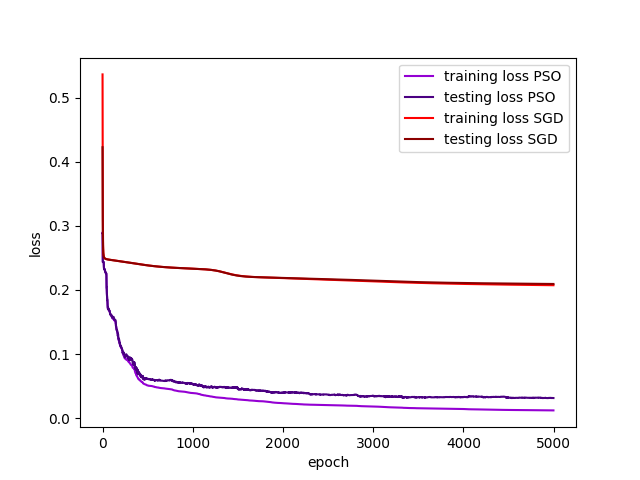
\includegraphics[scale=0.45]{figures/linear.png}    
      \end{center}                                                                                              
\end{figure}
The corresponding table detailing the final losses and fitness is in appendix A.2.
The restriction to linear inputs was not favourable for the SGD model which performed significantly worse in all aspects when compared to its nonlinear counterpart. 
The PSO model; however, performed nearly equally as well as its nonlinear counterpart.
It should be noted though that when using the provided tensorflow playground code, the SGD model performs about as well as the PSO model here.
With the architecture provided, we could argue that there really is no particular need to introduce nonlinear inputs into the model; however, by allowing nonlinear transformations to the data point, we are able to introduce curved aspects into the model earlier. This allows the model to better fit the data without increasing the complexity by needing extra hidden layers.  
\subsection{The Effect of Particle Swarm Parameters}
For this part of the task, we took a look at how changing various parameters affected the final training and testing errors, as well as the overall fitness of the model. The table showing these results is in appendix A.3 and A.4.
First, we took a look at varying $\omega$, considering $\omega = \{0.1, 0.2, \ldots, 0.9\}$. Here it is helpful to remember that $\omega$ represents the inertia of the particle. Too small, and the particles would have trouble moving, being guided primarily by the personal and global bests. Too much and the particle would have a hard time changing direction when the swarm dictates it to. One would expect the optimal $\omega$ to be somewhere near the middle then, and indeed our results show that the best $\omega = 0.7$, earning the network a fitness of 0.9208. 

While $\omega$ concerns itself with the velocity term, the parameters $\alpha_1$ and $\alpha_2$ help determine the weight of the personal and global bests in comparison to the particles current position.
We ran a similar experiment varying the value of $\alpha$ between 1.2 and 2.1. We decided for the sake of simplicity to follow convention and keep $\alpha_1=\alpha_2$. The table with this data is also in the appendix. The difference between the fitness of each model as we change the $\alpha$ parameter is much smaller than when we changed $\omega$. Furthermore, while changes in $\omega$ appeared to provide a smoother change in the fitness, changes in the $\alpha$ term do not, meaning that it would be much harder to choose properly. It stands to reason that the higher the value of $\alpha$, the more volatile the particle's movements will be, unless the particle is close to the optimal position. So a higher $\alpha$ would allow the possibility for a particle to overshoot the optimal position. In contrast, too low an $\alpha$ and the particle would be guided only by its inertia. Again, logically the best place to start looking then would be a median point between the two extremes. The table in appendix A shows that the $\alpha$ value with the best fitness is $\alpha=1.5$, which does fit with our hypothesis. This is a heuristic for where to start looking rather than a definitive guide. From this, one could draw the conclusion that extreme values for these parameters would almost never provide an optimal solution for this problem, and that it would be better to start with a more moderate value for each and adjust accordingly (or even better, use a MHO algorithm to find the optimal parameters).

\section{Genetic Algorithm (GA) to Optimize Shape of Neural Network}
The stochastic gradient descent(SGD)-based training seemed to outperform the PSO training in the training speed. Therefore, we chose to continue with SGD in the next tasks. While performing the tasks, we were able to significantly improve the SGD-based training performance so that $e_{test}<0.01$ could be consistently found within 5000 epochs using a tanh activation function and a learning rate of 0.3 for a network of shape (6,6,5,2,1). The following results are based on this starting point. For the genetic algorithm implementation, we modified an available genetic algorithm python library\footnote{Ryan (Mohammad) Solgi, \textbf{geneticalgorithm}: https://github.com/rmsolgi/geneticalgorithm} to accept an initial population seed and suppress some outputs that caused errors. The algorithm uses roulette wheel selection, point mutations, and uniform crossovers. Further details of running the implementation are available in the README for Task 2.

\subsection{Evolving the Neural Network Shape}
We designed a neural network creator using PyTorch that accepts a list of integers $[a_1,a_2,...,a_n]$ and encodes the list into a neural network where each entry in the list defines a layer of the network. The first and last elements of the list were selected to be 6 and 1 respectively, representing the six inputs ($x_1$, $x_2$, $x_1^2$, $x_2^2$, $\sin x_1$, $\sin x_2$) and one classification output. The list was limited to 6 elements of $x \in \{0,\ldots,8\}$, meaning four hidden layers of up to eight neurons each could be specified for the network. A layer length of 0 signifies a missing layer, allowing the network shape to be modular between 0 and 4 hidden layers. This level of complexity for the neural network is sufficient based on preliminary experiments.

A fitness function was designed to calculate the loss for a given shape that penalizes both prediction errors and increasing complexity of the neural network. For a neural network shape of $(a_n)_{n=1}^{l}$ where $l\in\mathbb{N}$ defines the number of layers, and each $a_n \in \mathbb{N}$ defines the number of neurons in layer $n$, the fitness function is as follows: 
\begin{equation}
	 f(e_{train,i},e_{test,i},a_n) = 1000\frac{\min_i (e_{train,i} + e_{test,i})}{2} + \sum_{n=1}^{l} a_n + 2n
\end{equation}
Here, $e_{train,i}$ and $e_{test,i}$ define the training and testing errors, respectively for each run of the NN. Within each neural network weight optimization by SGD, only the training loss defined by a mean-squared error was used. Furthermore, the $i$ subscript denotes which run was used, since for each NN shape, the weights were optimized twice to reduce the effect of variations due to the random initialization of the weights by PyTorch. The training and testing errors were scaled by 1000 to reflect their importance to the function.

Additionally, two termination criteria were included in the SGD optimization of the neural network to reduce solution times. First, if $e_{test}-e_{train}>0.1$, the optimiser terminated early and returned a large loss. Secondly, if $e_{test}<0.01$, the optimiser terminated immediately signaling a sufficiently low error and a successful training. 

\subsection{Effect of Genetic Algorithm Parameters}
The parameters considered to be of importance in the present genetic algorithm tuning were: elitism, mutation probability, and crossover probability. A population size of 30 was used to limit the solution time when the genetic algorithm was run for 100 generations. The figure below shows the effect of changing these parameters, with the exact parameter values and best results available in Appendix A.5.
\begin{figure}[h]                   
      \begin{center}                  
          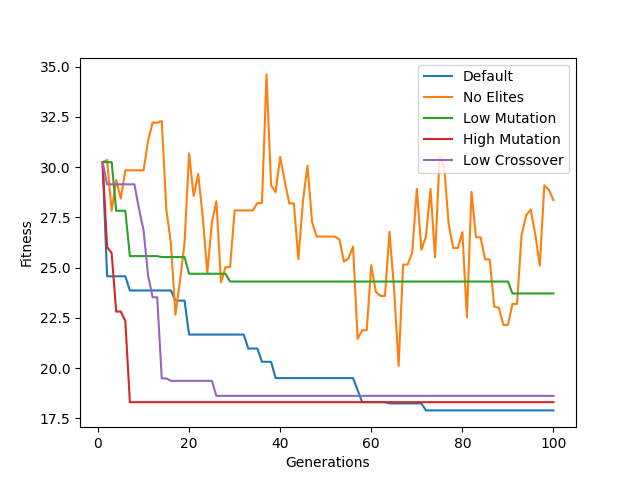
\includegraphics[scale=0.45]{figures/GA_diff_params.png}    
      \end{center}                                                                             
\end{figure}
Interestingly, the default parameters suggested by the author of the original GA code seem to perform very well and provide the best solution in our trials. We changed parameters to see what effect they have for a given initial population. From our results, we saw that elitism encouraged exploitation and ensured a good solution is reached more quickly. Without an elite in the population, there was a possibility of losing the information gained in previous generations and having an answer highly dependent on chance from one generation to another as is clearly visible in the plot above. This could be somewhat mitigated by having a larger population, but due to the long solution times, we did not try larger populations.

In the case of the mutation parameter, the solution seems to stagnate at a high error due to the lack of diversity in the population when mutation probability was very low. High mutation probability produced a reasonable result very quickly, but the algorithm had essentially been reduced to a random search at that point. While the no-free-lunch theorem implies that this approach is valid for average performance, our aim is to use metaheuristic optimization to produce better results. Lowering crossover seems to have a similar effect on the final answer, but more generations were needed to produce the best solution compared to the high mutation case. High crossover, as was true in the default case, seems to only marginally improve the solution, indicating that the algorithm may work well with just mutations, but not as high mutations as to result in a random search. It should be noted that the randomness of the mutations and crossovers can result in different final answers for identical inputs and initial populations, so better conclusions about the effect of the parameters should be made by averaging several runs together if possible. 

\subsection{Best Neural Network}
The best neural network according to the simulation was $(6,6,0,1,0,1)$. After dropping the 0 elements, this shape essentially denotes that with the linear, squared, and sine terms, the network can achieve an $e_{test}<0.01$ with two hidden layers, one with 6 neurons, and another with just 1. 
The second, 1-neuron hidden layer is interesting because further manual tests with a shape of $(6,6,1)$ show that $e_{test}<0.01$ in 3 out of 100 training runs of 5000 epochs each. So, even if the GA guessed that shape, there is a high probability it was ignored due to high loss. It should be noted that the goal of the optimization was to generate the simplest network that captured the spiral features well. The difficulty of obtaining the weights for a given shape was not a focus and was only indirectly captured in the fitness function due to the randomness of the training. Slightly larger network of shapes like $(6,8,2,1)$ achieved $e_{test}<0.01$ much faster and more consistently than $(6,6,1)$. 

\section{Controlling the Neural Network Structure with Genetic Programming}
In the previous task, we showed that a neural network with a single hidden layer sufficiently captures the spiral features in the dataset. The goal of this task is to explore some different configurations for the network.
\subsection{Operators and Parameters}
The genetic program accepts the following activation functions: [torch.tanh, torch.sin, torch.sigmoid, torch.abs]. The torch.abs is a placeholder for the linear activation. Learning rates of [0.01 , 0.03, 0.1, 0.3] were allowed. We built the program upon the previous task, making the genetic algorithm able to accept variables of with different bounds. Each of the activation functions and learning rates was encoded into an integer sequence that represents the possible options that the genetic program could choose. Thus, the genetic program accepted two additional elements of $x \in \{0,\ldots,3\}$ beyond the  the GA. Further details of the implementation are in the README for task 3. The same fitness function as in the previous task was used to optimize the genetic program.
\subsection{Genetic Program Results}
In the previous task, we showed that crossover was useful but not necessary in the genetic algorithm if mutation was used properly. Here, we decided to test if 4-5 member populations produce good results. Our results were rather inconsistent with just 5 members. The results seem highly dependent on the initial population/training luck and did not produce results better than those found in the "Default" trial in the previous section. We used the same criteria for fitness as before where we try to find the neural network with the fewest hidden layers and neurons. 

The poor results are not surprising as there is not much variability needed when the network can be satisfied with a single hidden layer as discussed in the previous task. Tanh and sin activation functions seem to perform equally well. The sigmoid function did not produce good results, and the linear function was already shown to have poor performance in the first task. A learning rate of 0.3 was optimal for reaching a small $e_{test}$ within the specified 5000 epochs for training. Higher training rates than 0.3 resulted in a lot of fluctuations. Manual testing with the smaller learning rates showed that the training and test losses were still steadily decreasing after 5000 epochs, so a longer training time should produce better results but was not tested due to the long solution times. However, overall, the results also suffered due to the small population size that did not allow for much diversity in the limited epochs.

\subsection{Outlook on Additional Tasks}
There are several methods of improving the current results and also implementing new features.
\begin{itemize}
    \itemsep0em 
    \item For the PSO, using a constriction factor could encourage faster convergence of the PSO swarm and improve algorithm performance compared to SGD.
    \item Implementing regularization and/or "bouncing" of the PSO particles from a boundary can be used to reduce the likelihood of a divergent particle swarm.
    \item For the PSO, GA, and GP, it may be useful to implement a low-level algorithm like hill climbing or gradient descent as an added stage in the optimization, in essence simulating the Baldwin effect. 
    \item The genetic program can be improved to consider different types of features for each hidden layer to increase the diversity of possible solutions.
    \item Parallelizing some computations, especially those that lend to it naturally like evaluations of members in a given generation of a GA or evaluations of a particles in a PSO, can improve solution times of the algorithms.
\end{itemize}  
  

\pagebreak
\appendix
\section{Tables and Figures}
\subsection{Results of experiment with nonlinear inputs for PSO and SGD optimised neural networks:}
\begin{center}
 \begin{tabular}{||c c c c||} 
 \hline
 Optimiser & Average Training Loss & Average Testing Loss & Average Fitness \\ [0.5ex] 
 \hline\hline
 PSO & 0.0121 & 0.0298 & 0.9612 \\ 
 \hline
 SGD & 0.0398 & 0.0463 & 0.9503 \\
 \hline
\end{tabular}
\end{center}
\subsection{Results of experiment with linear inputs for PSO and SGD optimised neural networks:}
\begin{center}
 \begin{tabular}{||c c c c||} 
 \hline
 Optimiser & Average Training Loss & Average Testing Loss & Average Fitness \\ [0.5ex] 
 \hline\hline
 PSO & 0.0262 & 0.0419 & 0.9501 \\ 
 \hline
 SGD & 0.1982 & 0.2007 & 0.7981 \\
 \hline
\end{tabular}
\end{center}
\subsection{Results of experiments with varying $\omega$ ($\alpha_1=\alpha_2=1.6$):}
\begin{center}
 \begin{tabular}{||c c c c||} 
 \hline
 $\omega$ & $e_T$ & $e_\tau$ & $f$ \\ [0.5ex] 
 \hline\hline
 0.1 & 0.2372 & 0.2975 & 0.6723 \\ 
 \hline
 0.2 & 0.1946 & 0.2733 & 0.6873 \\
 \hline
 0.3 & 0.1467 & 0.195 & 0.7808 \\
 \hline
 0.4 & 0.1823 & 0.252 & 0.7131 \\
 \hline
 0.5 & 0.0928 & 0.1714 & 0.7893 \\
 \hline
 0.6 & 0.0129 & 0.0629 & 0.9121 \\
 \hline
 0.7 & 0.0097 & 0.056 & 0.9208 \\
 \hline
 0.8 & 0.1976 & 0.2541 & 0.7176 \\
 \hline
 0.9 & 0.4023 & 0.2909 & 0.542 \\
 \hline
\end{tabular}
\end{center}
\subsection{Results of experiments with varying $\alpha$ ($\omega=0.7$):}
\begin{center}
 \begin{tabular}{||c c c c||} 
 \hline
 $\alpha$ & $e_T$ & $e_\tau$ & $f$ \\ [0.5ex] 
 \hline\hline
 1.2 & 0.027 & 0.0987 & 0.8654 \\ 
 \hline
 1.3 & 0.0297 & 0.0683 & 0.9124 \\
 \hline
 1.4 & 0.0163 & 0.1015 & 0.8559 \\
 \hline
 1.5 & 0.0064 & 0.0214 & 0.9711 \\
 \hline
 1.6 & 0.024 & 0.1602 & 0.7718 \\
 \hline
 1.7 & 0.029 & 0.1351 & 0.8118 \\
 \hline
 1.8 & 0.0158 & 0.0395 & 0.9481 \\
 \hline
 1.9 & 0.1669 & 0.2009 & 0.7821 \\
 \hline
 2.0 & 0.2168 & 0.2032 & 0.8036 \\
 \hline
 2.1 & 0.2691 & 0.122 & 0.9515 \\
 \hline
\end{tabular}
\end{center}
\subsection{Results of experiment with different genetic algorithm parameters for shape determination:}
Each trial had a population size of 30 and was run for 100 epochs. The algorithm uses roulette wheel selection, point mutations, and uniform crossovers. A parent ratio of 0.3 was used for all trials.
\begin{center}
 \begin{tabular}{||c c c c c c||} 
 \hline
 Trial & \# Elites & Crossover & Mutation & Fitness & Shape\\ [0.5ex] 
 \hline
 \hline
 Default & 1 & 0.5 & 0.1 & 16.90 & (6,6,0,1,0,1) \\ 
 \hline
 No Elites & 0 & 0.5 & 0.1 & 20.11 & (6,7,1,1,0,1) \\
 \hline
 Low Mutation & 1 & 0.5 & 0.001 & 23.71 & (6,4,6,3,0,1) \\
 \hline
 High Mutation & 1 & 0.5 & 0.5 & 18.31 & (6,6,0,2,0,1) \\
 \hline
 Low Crossover & 1 & 0.01 & 0.1 & 18.62 & (6,6,0,3,0,1) \\
 \hline
\end{tabular}
\end{center}


\end{document}